\usetikzlibrary{shapes,fit}
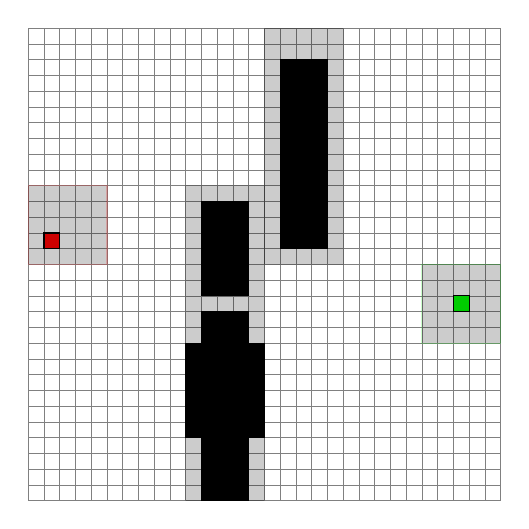
\begin{tikzpicture}%[node distance = 3cm, auto,scale=0.85, every node/.style={scale=0.85}]
% Place nodes
\centering

\draw[step=0.2cm,gray,very thin] (0,0) grid (6,6);

\filldraw[fill=red] (0.2, 3.2) rectangle (0.4, 3.4);

\filldraw[fill=green] (5.4, 2.4) rectangle (5.6,2.6);

\filldraw[fill=black] (2.2, 0) rectangle (2.8, 2.4); %bottom left
\filldraw[fill=black] (2, 0.8) rectangle (3, 2); %bottom left

\filldraw[fill=black] (2.2, 2.6) rectangle (2.8, 3.8 ); %upper left

\filldraw[fill=black] (3.2 , 5.6) rectangle (3.8, 3.2); %upper right



\filldraw[draw=red, opacity=0.2] (0,3) rectangle (1,4);

\filldraw[draw=green, opacity=0.2] (5,2) rectangle (6,3);

\filldraw[draw=black, opacity=0.2] (2,0) rectangle (3,4);
\filldraw[draw=black, opacity=0.2] (3,6) rectangle (4,3);


\end{tikzpicture}